\chapter{Lattice Boltzmann method}\label{lbm}

A fluid can be described as a continuum and using a macroscopic perspective, where it is treated as a whole, and its state is characterized by macroscopic quantities such as density, flow velocity, or pressure. In this case the governing equations are the Navier-Stokes equations \eqref{NS}. A fluid's behavior can also be described on a microscopic scale by tracking the dynamics of all individual particles. A significant drawback of this approach is its evident computational complexity, which is directly proportional to the number of particles involved.

A compromise between these two approaches is the description of a fluid on a mesoscopic scale \cite{PE}, which is based on the kinetic theory. The fluid is described using one-particle density function \( f(\vec{x},\vec{\xi}, t) \) \si{[kg.s^3.m^{-6}]}, which describes the system in the space of positions \( \vec{x} \) and microscopic velocities \( \vec{\xi} \), and time \( t \). The density functions  represent the density of particles at a position \( \vec{x} \), with microscopic velocity \( \vec{\xi} \), at time \( t \).

The one-particle density functions satisfy the Boltzmann transport equation \cite{Kruger}
\begin{equation}\label{eq:BTR}
	\frac{\partial f}{\partial t} + \sum_{i = 1}^{3} \xi _{i} \frac{\partial f}{\partial x_{i}} + \sum_{i = 1}^{3} g_{i} \frac{\partial f}{\partial \xi _{i}} = \mathcal{C}(f), 
\end{equation}
where \( \vec{g} \) \si{[m.s^{-2}]} is the acceleration vector of external forces, and \( \mathcal{C}(f)\) \si{[kg.s^2.m^{-6}]} is the collision operator.

Using the distribution functions \( f \), certain macroscopic quantities can be expressed as statistical moments \cite{Kruger}, such as

\begin{subequations}\label{eq:macroscopic basic}
	\begin{alignat}{1}
		\rho(\vec{x}, t) & =\int\displaylimits_{\mathbb{R}^3} f(\vec{x}, \vec{\xi}, t) \mathrm{~d} \vec{\xi} \label{subeq:rho}, \\
		\rho(\vec{x}, t) \vec{u}(\vec{x}, t) & =\int\displaylimits_{\mathbb{R}^3} f(\vec{x}, \vec{\xi}, t) \, \vec{\xi} \mathrm{~d} \vec{\xi} \label{subeq:momentum}.
	\end{alignat}
\end{subequations}


The lattice Boltzmann method (LBM) is a numerical method based on the mesoscopic description of fluids. The numerical scheme of LBM can be derived by discretizing \eqref{eq:BTR}. In LBM, the spatial discretization is performed using a discrete equidistant lattice, and the discretization of velocity space utilizes a finite set of discrete microscopic velocities. These discrete velocity sets are described using velocity models denoted as D$d$Q$q$, where $ d$  specifies the spatial dimension and $q$ the number of different velocity directions at each lattice node.

In this thesis, we use the D3Q27 velocity model illustrated in Figure~\ref{fig:d3q27}.

\begin{figure}[h]
	\centering
	\vspace{4mm}
	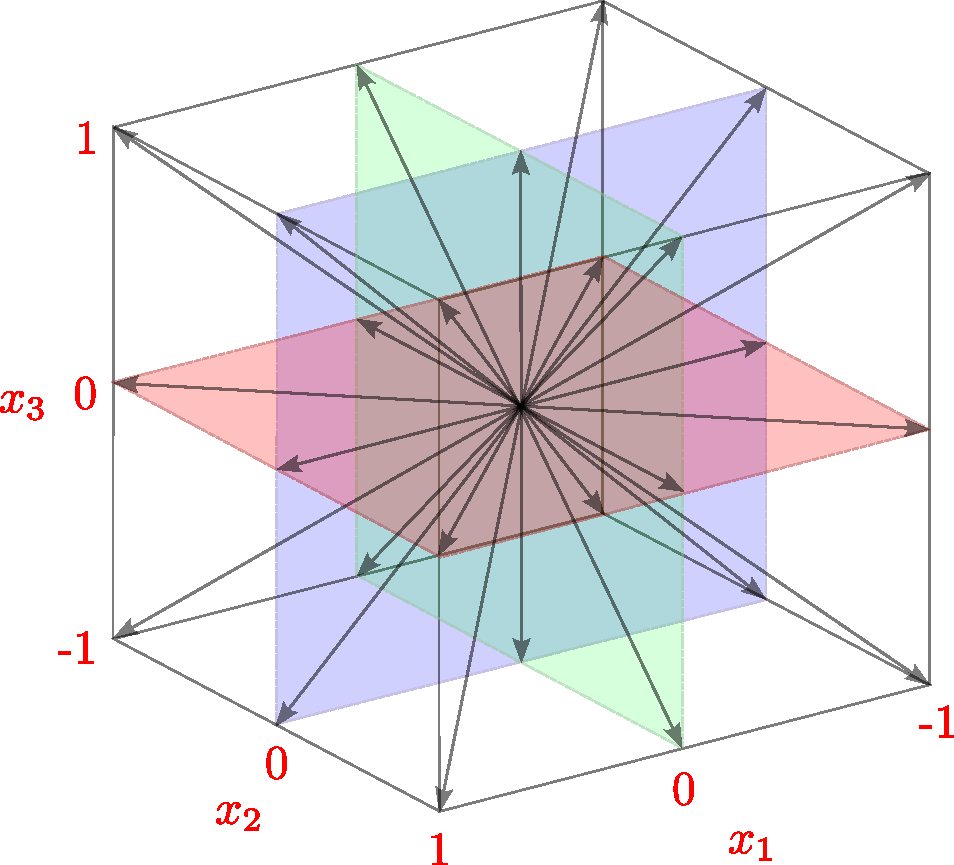
\includegraphics[width=.6\textwidth]{figures/d3q27.pdf}
	\caption{Geometric representation of the D3Q27 velocity model.}
	\label{fig:d3q27}
\end{figure}

In the case of the D3Q27 model, the velocity space is discretized by a finite set of microscopic velocities defined as

\begin{equation}\label{eq:velocities}
	\begin{aligned}
		\left(\boldsymbol{\xi}_k\right)_{k=1}^{27} = &
		\left(
		\begin{aligned}
			&\left(
			\begin{aligned}
				0 \\ 0 \\ 0
			\end{aligned}
			\right),
			\left(
			\begin{aligned}
				1 \\ 0 \\ 0
			\end{aligned}
			\right),
			\left(
			\begin{aligned}
				0 \\ 1 \\ 0
			\end{aligned}
			\right),
			\left(
			\begin{aligned}
				0 \\ 0 \\ 1
			\end{aligned}
			\right),
			\left(
			\begin{aligned}
				-1 \\ 0 \\ 0
			\end{aligned}
			\right),
			\left(
			\begin{aligned}
				0 \\ -1 \\ 0
			\end{aligned}
			\right),
			\left(
			\begin{aligned}
				0 \\ 0 \\ -1
			\end{aligned}
			\right),
			\left(
			\begin{aligned}
				0 \\ 1 \\ 1
			\end{aligned}
			\right),
			\left(
			\begin{aligned}
				0 \\ 1 \\ -1
			\end{aligned}
			\right),
			\left(
			\begin{aligned}
				0 \\ -1 \\ 1
			\end{aligned}
			\right),
			\left(
			\begin{aligned}
				0 \\ -1 \\ -1
			\end{aligned}
			\right),
			\left(
			\begin{aligned}
				1 \\ 1 \\ 0
			\end{aligned}
			\right),
			\left(
			\begin{aligned}
				1 \\ -1 \\ 0
			\end{aligned}
			\right),
			\left(
			\begin{aligned}
				-1 \\ 1 \\ 0
			\end{aligned}
			\right), \\
			&\left(
			\begin{aligned}
				-1 \\ -1 \\ 0
			\end{aligned}
			\right),
			\left(
			\begin{aligned}
				1 \\ 0 \\ 1
			\end{aligned}
			\right),
			\left(
			\begin{aligned}
				1 \\ 0 \\ -1
			\end{aligned}
			\right),
			\left(
			\begin{aligned}
				-1 \\ 0 \\ 1
			\end{aligned}
			\right),
			\left(
			\begin{aligned}
				-1 \\ 0 \\ -1
			\end{aligned}
			\right),
			\left(
			\begin{aligned}
				1 \\ 1 \\ 1
			\end{aligned}
			\right),
			\left(
			\begin{aligned}
				1 \\ 1 \\ -1
			\end{aligned}
			\right),
			\left(
			\begin{aligned}
				1 \\ -1 \\ 1
			\end{aligned}
			\right),
			\left(
			\begin{aligned}
				1 \\ -1 \\ -1
			\end{aligned}
			\right),
			\left(
			\begin{aligned}
				-1 \\ 1 \\ 1
			\end{aligned}
			\right),
			\left(
			\begin{aligned}
				-1 \\ 1 \\ -1
			\end{aligned}
			\right),
			\left(
			\begin{aligned}
				-1 \\ -1 \\ 1
			\end{aligned}
			\right),
			\left(
			\begin{aligned}
				-1 \\ -1 \\ -1
			\end{aligned}
			\right)
		\end{aligned}
		\right).
	\end{aligned}
\end{equation}



\section{Non-dimensionalization and discretization}
The computational domain \( (0 ; L_1) \times(0 ; L_2) \times(0 ; L_3)\), where \( L_i\) \si{[m]}, $i=1,2,3$, represent the dimensions of the domain, is discretized using an equidistant grid with a spatial step size \( \Delta l \) \si{[m]}. The time interval is discretized uniformly using a time step size \( \Delta t \)~\si{[s]}.

In LBM, it is common to work with non-dimensional quantities instead of physical ones, as discussed in \cite{Kruger}. This section introduces the conversion relationships for transitioning to a non-dimensional system, defines the lattice used for domain discretization, and describes the discretized Boltzmann transport equation.

\subsection{Non-dimensional units}
The transition between unit systems can be performed using the law of similarity for fluid dynamics, which ensures that the values of relevant non-dimensional quantities remain constant \cite{Kruger}. One such non-dimensional quantity that can be used during the transition is, for example, the Reynolds number \eqref{Re}. It should be emphasized that the physical principles remain valid regardless of the choice of the unit system. 

In the following conversion relations, all quantities in lattice units are marked with the superscript \( L \). It can be shown \cite{Kruger} that the following holds:
\begin{eqnarray}
	l^{L}_0 &=& \dfrac{l_{0}}{\Delta l},\\[5pt]
	t^{L}_0 &=& \dfrac{t_{0}}{\Delta t},\\[5pt]
	\nu^L &=& \nu \dfrac{\Delta t}{\Delta l^{2}},\\[5pt]
	u^{L}_{i} &=& \dfrac{\Delta t}{\Delta l} u_{i}, \ i \in \{1, 2, 3\}.
\end{eqnarray}
The characteristic length, time, and velocity values are chosen based on the given physical problem. The computational domain's largest dimension or the size of an obstacle within the flow is typically chosen as \( l_{0} \). Detailed derivations of these relations can be found in \cite{Kruger}. From the relationship for kinematic viscosity, it can be seen that for a given spatial step \( \Delta l \), the time step \( \Delta t \) is linked to the value of \( \nu^L \).

For simplicity, in this work, we will assume that the spatial step \( \Delta l ^L \) and the time step \( \Delta t ^L \) in lattice units are \( \Delta l ^L  =  \Delta t ^L = 1 \). In the remainder of this chapter, we use lattice units exclusively and for brevity we omit the superscript \( L \), though all quantities will be non-dimensional.
\subsection{Computational Domain and Discrete Grid}
From this point forward, we assume that all quantities are expressed in lattice units, meaning $ \Delta l $ and $ \Delta t $ now represent non-dimensional spatial and time steps, respectively. We consider a cuboidal computational domain $ \Omega \subset \mathbb{R}^3 $, see section \ref{pred}. This domain in LBM is discretized using an equidistant grid

\begin{subequations}\label{eq:domain}
	\begin{eqnarray}
		&\hat{\Omega} = \left\{ \vec{x}_{i,j,k} = (i \Delta l,\,j \Delta l, \,k \Delta l)^T \ \middle| \ i \in \{1, \dots, N_{1} - 1\}, j \in \{1, \dots, N_{2} - 1 \}, k \in \{1, \dots, N_{3} - 1 \} \right\},\\[4pt]
		&\overline{\hat{\Omega}} = \left\{ \vec{x}_{i,j} = (i \Delta l,\,j \Delta l)^T \ \middle| \ i \in \{0, \dots, N_{1} \}, j \in \{0, \dots, N_{2} \}, k \in \{0, \dots, N_{3} \} \right\},
	\end{eqnarray}
\end{subequations}
where $ N_{i} $ [-] denotes the number of grid points in the $ x_i $ direction, $ i = 1, 2, 3 $.

The boundary of the domain $ \Omega $ will be denoted by $ \partial \Omega $ and understood as the closure of the disjoint union of the individual parts 
\begin{equation}\label{eq:border decomposition}
	\partial \Omega = \overline{\partial \Omega_{\mathrm{W}} \cup \partial \Omega_{\mathrm{E}} \cup \partial \Omega_{\mathrm{N}} \cup \partial \Omega_{\mathrm{S}} \cup \partial \Omega_{\mathrm{F}} \cup \partial \Omega_{\mathrm{B}}},
\end{equation}
where the meanings of $\partial \Omega_{\mathrm{W}} , \partial \Omega_{\mathrm{E}} , \partial \Omega_{\mathrm{N}}, \partial \Omega_{\mathrm{S}}, \partial \Omega_{\mathrm{F}}$, $  \partial \Omega_{\mathrm{B}} $ are illustrated in Figure \ref{fig:domain}. We will further consider the discretization of the boundary of the computational domain as
\begin{equation}\label{eq:border}
	\partial\hat{\Omega} = \overline{\hat{\Omega}} \, \backslash \, \hat{\Omega},
\end{equation}
with the corresponding parts of the discrete boundary denoted as $ \partial \hat{\Omega}_{\mathrm{W}} , \partial \hat{\Omega}_{\mathrm{E}} , \partial \hat{\Omega}_{\mathrm{N}}, \partial \hat{\Omega}_{\mathrm{S}}, \partial \hat{\Omega}_{\mathrm{F}}$,  and $ \partial \hat{\Omega}_{\mathrm{B}} $.
\begin{figure}[H]
	\centering
	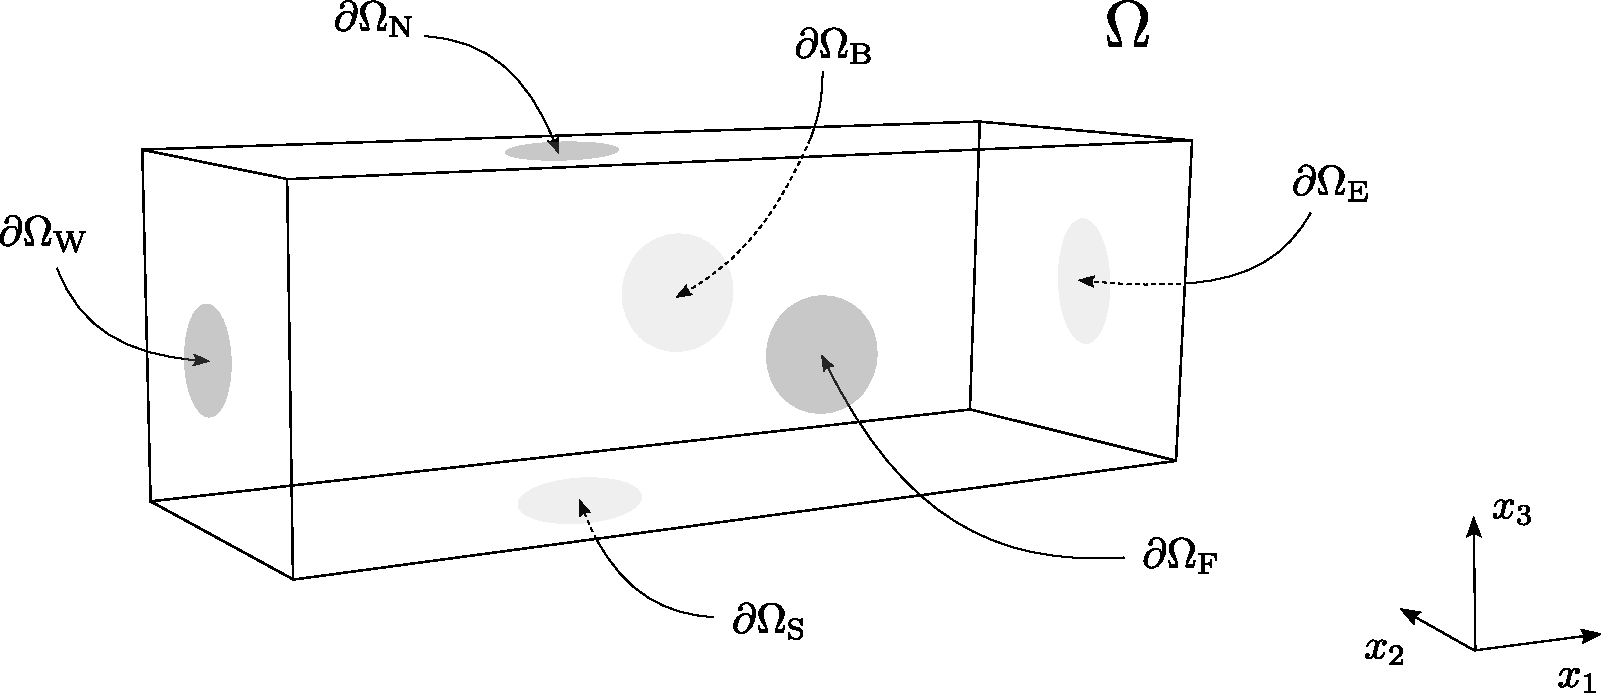
\includegraphics[width=0.99\textwidth]{figures/omega.pdf}
	\caption{Schematic representation of the computational domain $ \Omega $ and its boundary $ \partial \Omega $.}  
	\label{fig:domain}
	\vspace{1.8mm}
\end{figure}

The time interval over which the problem will be investigated will be denoted by $ \mathcal{I} $ , where ${\mathcal{I} = \langle 0, T \rangle}$, and $ T > 0 $. The interval $ \mathcal{I} $ is discretized as
\begin{equation}\label{eq:timediscrete}
	\hat{\mathcal{I}} = \left\{ t_{i} = i \frac{T}{N_t} \ \middle| \ i \in \left\{0, \dots, N_{t} \right\} \right\},
\end{equation}
where $ N_t $ represents the number of discrete time steps for the discretization of the interval $ \mathcal{I} $.

\subsection{Discrete Boltzmann transport equation}
When using the D3Q27 model, we work with a set of distribution functions
\begin{equation}\label{eq:ddfs}
	\left\{ f_k (\vec{x}, t) \ \middle| \ k = 1, \dots, 27 \right\}, \ \forall \vec{x} \in \hat{\Omega}, \ \forall t \in \hat{\mathcal{I}},
\end{equation}
where the indices correspond to the directions of microscopic velocities from \eqref{eq:velocities}.

It can be shown that by discretizing the equation \eqref{eq:BTR}, we obtain the form
\begin{equation}\label{eq:BTRdiscrete}
	f_{k}\left(\vec{x}+\Delta t \vec{\xi}_{k}, t+\Delta t \right) =
	f_{k}(\vec{x}, t) + \mathcal{C}_{k}(\vec{x}, t) + \mathcal{S}_{k}(\vec{x}, t), \hspace{2.5mm} k \in \{1, \dots, 27 \}, \ \forall \vec{x} \in \hat{\Omega}, \ \forall t \in \hat{\mathcal{I}},
\end{equation}
where $ \mathcal{C}_{k} $ represents the discrete collision operator and $ \mathcal{S}_{k} $ is the discrete forcing term. Details of the derivation of the discrete form of the Boltzmann transport equation can be found in \cite{Kruger}.

The discrete collision operator $\mathcal{C}_{k}$ in equation \eqref{eq:BTRdiscrete} defines the specific variant of LBM. Several choices for $\mathcal{C}_{k}$ exist, each corresponding to different LBM formulations. These include, for instance, the single relaxation time (SRT-LBM) \cite{GeierCuLBM}, multiple relaxation time (MRT-LBM) \cite{MRT}, central moment (CLBM) \cite{GeierCLBM}, entropic (ELBM) \cite{ELBM}, and cumulant-based (CuLBM) \cite{GeierCuLBM} approaches. In this work, we use the cumulant collision operator, as detailed in \cite{GeierCuLBM}.


We can further introduce the post-collision distribution functions $ f^{*}_{k} $ as
\begin{equation}\label{eq:fstar}
	f^{*}_{k}(\vec{x}, t) = f_{k}(\vec{x}, t) + \mathcal{C}_{k}(\vec{x}, t) + \mathcal{S}_{k}(\vec{x}, t), \hspace{2.5mm} k \in \{1, \dots, 27 \}, \ \forall \vec{x} \in \hat{\Omega}, \ \forall t \in \hat{\mathcal{I}}.
\end{equation}
Using $ f^{*}_{k} $, we can express \eqref{eq:BTRdiscrete} in the form
\begin{equation}\label{eq:collision}
	f_{k}\left(\vec{x}+\Delta t \vec{\xi}_{k}, t+\Delta t\right) = f^{*}_{k}(\vec{x}, t), \hspace{2.5mm} k \in \{1, \dots, 27 \}, \ \forall \vec{x} \in \hat{\Omega}, \ \forall t \in \hat{\mathcal{I}},
\end{equation}
which can be interpreted as an explicit prescription for calculating the distribution functions.
\subsection{Macroscopic Quantities}\label{macro}
Finally, we present the relations for calculating some of the macroscopic quantities. Some of these relations can be derived through the process of discretization from the general relations \eqref{eq:macroscopic basic} \cite{Kruger}. The relations for calculating density, momentum, and pressure are as follows:

\begin{subequations}\label{macroeq}
	\begin{eqnarray}
		\label{rho}
		\rho &=& \sum_{k=1}^{27} f_{k},\\[3pt]
		\rho \vec{u} &=& \sum_{k=1}^{27} f_{k} \vec{\xi_{k}} + \rho \dfrac{\Delta t}{2} \vec{g},\\[3pt]
		p &=& p_0 + c_{s}^{2} (\rho - \rho_0),
	\end{eqnarray}
\end{subequations}
where $ p_0 $ \si{[-]} is the non-dimensional reference value of pressure, $ c_s $ \si{[-]} is the non-dimensional (lattice) speed of sound, and $ \rho_0 $ is the non-dimensional reference value of density. For $ c_s $ in the D3Q27 model, $ c_s = \frac{1}{\sqrt{3}} $. Furthermore, we consider $ \rho_0 = 1 $. A detailed description of the calculation of macroscopic quantities is provided in \cite{Kruger}.
\section{LBM algorithm}\label{algoritmus LBM}
The LBM algorithm can be summarized in several steps:
\begin{enumerate}
	\item \textbf{Initialization} of initial conditions on the grid, discussed in section \ref{pocatecni a okrajove podminky}.
	\item \textbf{Cycle} ending with the fulfillment of a user-specified termination condition.
	\begin{enumerate}
		\item \textbf{Streaming} of post-collision distribution functions \( f^{*}_{k} \) in the respective directions \( \vec{\xi_{k}} \).
		\item \textbf{Calculation of macroscopic quantities} using the relations \eqref{macroeq}.
		\item \textbf{Collision}, where the post-collision state of the distribution function is calculated using \eqref{eq:collision}, and \textbf{application of boundary conditions}, discussed in section \ref{pocatecni a okrajove podminky}.
	\end{enumerate}
	\item \textbf{End of the algorithm.}
\end{enumerate}
A flowchart of the LBM algorithm is shown in Figure \ref{fig:algo}.
\begin{figure}[h]
	\centering
	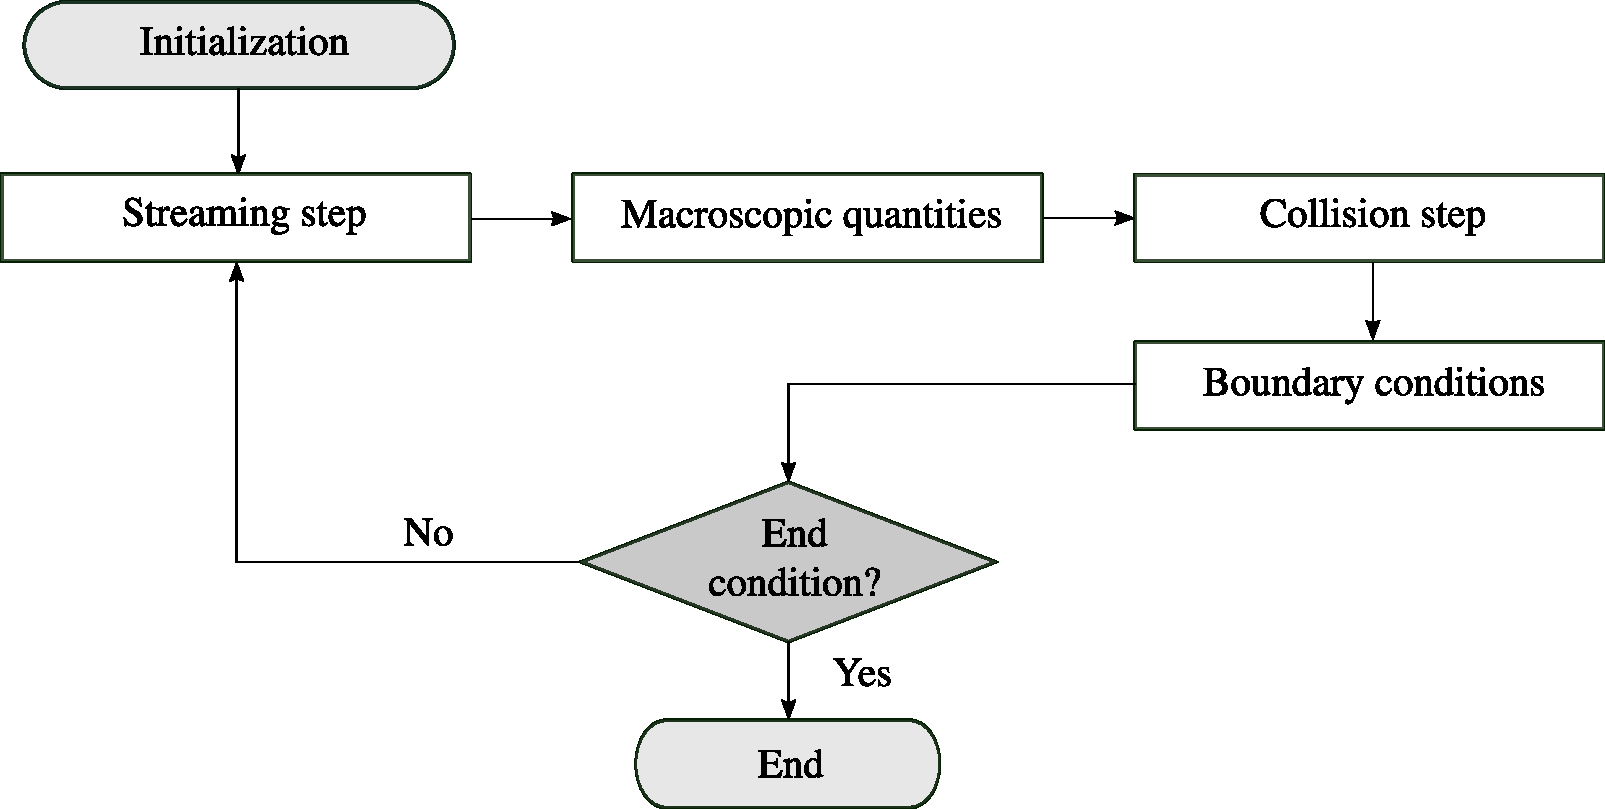
\includegraphics[width=0.78\textwidth]{figures/algo-bw.pdf}
	\caption{Flowchart of the LBM algorithm.}
	\label{fig:algo}
\end{figure}
\input{chapters/lbm/collision.tex}
\section{Initial and boundary conditions}\label{pocatecni a okrajove podminky}

The choice of initial and boundary conditions is an integral part of the lattice Boltzmann method to ensure consistency the mesoscopic description. Therefore, the chosen initial and boundary conditions are described in more detail in this section.

\subsection{Initial condition}\label{pocatecni podminka}
Let us now consider the domain defined by relations \eqref{eq:domain}. In this work, the equilibrium distribution function \( f^{\mathrm{eq}} \) is used to set the initial condition. The equilibrium distribution function is given by
\begin{equation}\label{eq:feq}
	f^{\mathrm{eq}}_{k} = \rho w_{k} \, \left(1 + \frac{\vec{\xi_{k}} \cdot \vec{u}}{c^{2}_{s}} + \frac{(\vec{\xi_{k}} \cdot \vec{u})^2}{2c^{4}_{s}} - \frac{\vec{u} \cdot \vec{u}}{2c^{2}_{s}} \right)\, , \hspace{2mm} k \in \{1,\dots,27\},
\end{equation}
where \( w_{k} \) are the weights specific to the chosen velocity model. For the D3Q27 model, these weights are defined as \cite{Kruger}
\begin{equation}
	w_k= \begin{cases}\frac{8}{27}, & k=1, \\ \frac{2}{27}, & k = 2,3, \ldots, 7, \\ \frac{1}{54}, & k = 8,9, \ldots, 19, \\ \frac{1}{216}, & k = 20,21, \ldots, 27.\end{cases}
\end{equation}
The initial density \( \rho \) and the velocity \( \vec{u} \), are denoted as \( \rho _{\mathrm{ini}} \) and \( \vec{u} _{\mathrm{ini}} \), respectively. At each lattice node \( \vec{x} \in \hat{\Omega} \) at time \( t=0 \), the distribution functions are initialized as
\begin{equation}\label{eq:initial condition}
	f^{}_{k} (\vec{x}, 0) = f^{\mathrm{eq}}_{k} (\rho _{\mathrm{ini}} (\vec{x}), \vec{u} _{\mathrm{ini}} (\vec{x})), \hspace{3mm} k \in \{1, \dots 27\}.
\end{equation}

This approach assumes that the non-equilibrium component of the distribution functions, defined as \( f^{\mathrm{neq}}_{k} = f_{k} - f^{\mathrm{eq}}_{k} \), can be neglected, and the distribution functions can be approximated by their equilibrium part. A significant advantage of this choice of initial condition approximation is its easy implementation. While more advanced initialization methods exist  \cite{PE}, the equilibrium-based approach is used in this work.

\subsection{Boundary conditions}


\subsubsection*{Bounce-back boundary condition}\label{bounce-back}
The first boundary condition discussed is the bounce-back boundary condition, specifically its \textit{fullway} variant \cite{Kruger}. The bounce-back boundary condition is typically used for modeling the interface between a fluid and a solid. Its advantage is that it satisfies the no-slip condition at the fluid-solid interface while remaining straightforward to implement. The principle of the bounce-back boundary condition is that at the interface, the distribution functions corresponding to particles with microscopic velocity \( \vec{\xi_{k}} \) are reflected back into the directions from which they arrived at the node, with velocity \( \vec{\xi_{\bar{k}}} = -\vec{\xi_{k}} \).

When using this boundary condition, the fluid-solid interface is located halfway between the fluid and solid nodes. For curved boundaries that are not parallel to the grid, the bounce-back method leads to a "staircase" shape of the boundary, which can limit the accuracy of the simulation.

In this approach, particles are reflected over two time steps. During this time, the particles reach the solid nodes, where their direction is reversed and they are streamed back, as schematically shown in Figure \ref{fig:fbb}.

\begin{figure}[h]
%	\vspace{-.5cm}
	\centering

	\begin{subfigure}{0.48\textwidth}
		\centering
		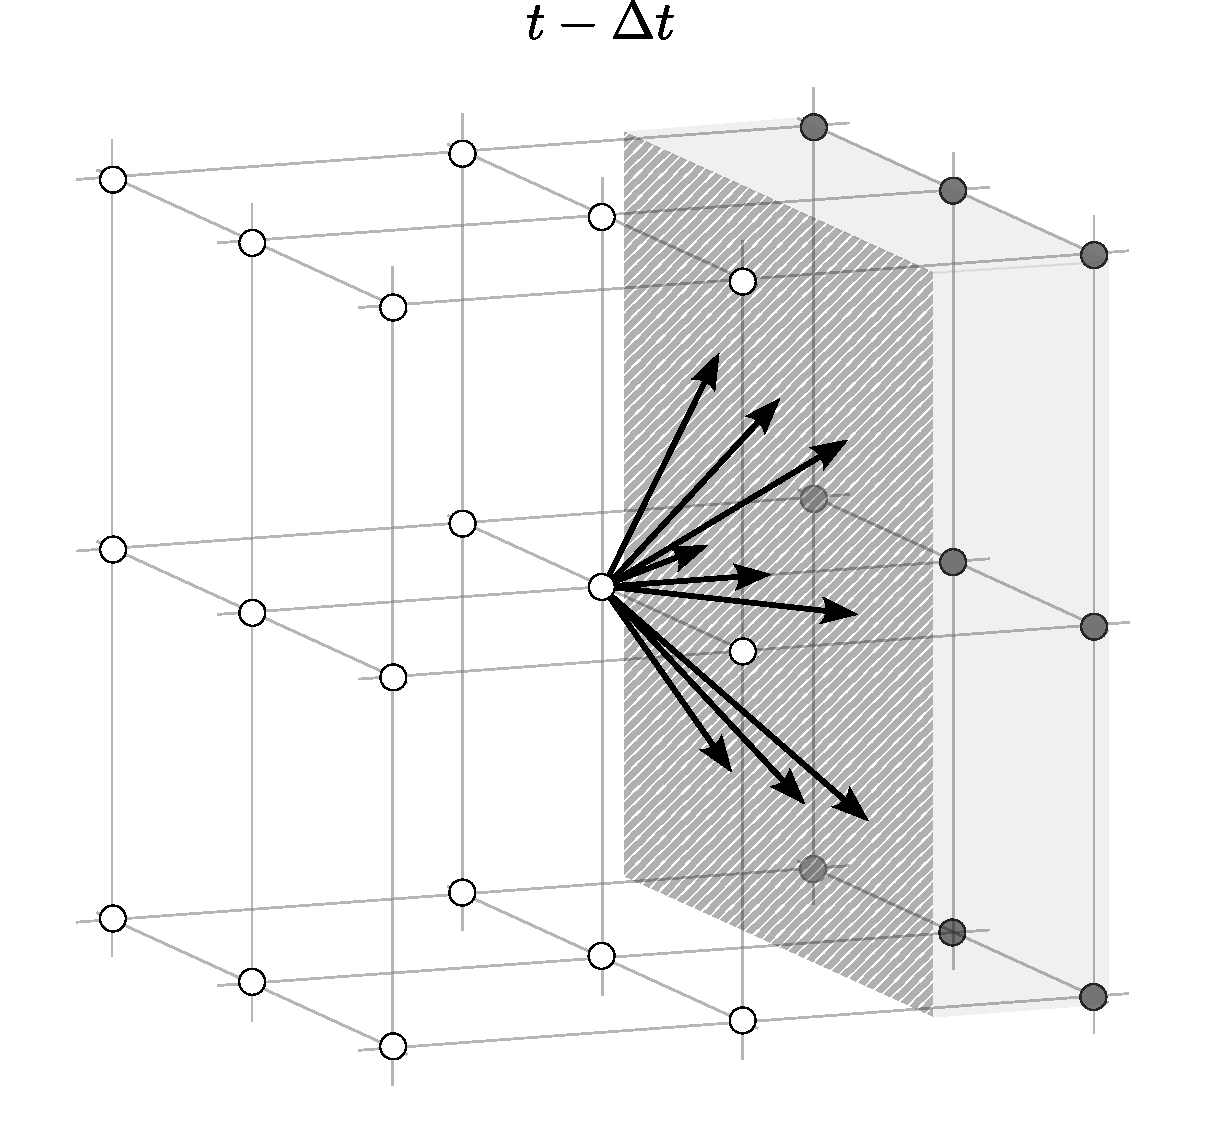
\includegraphics[width=0.9\textwidth, trim={0mm 0mm 0mm 0mm}]{figures/fwbba.pdf}
		\caption{Step before the streaming at time $t - \Delta t$.}
		\label{fig:bba}
	\end{subfigure}
	\begin{subfigure}{0.48\textwidth}
		\centering
		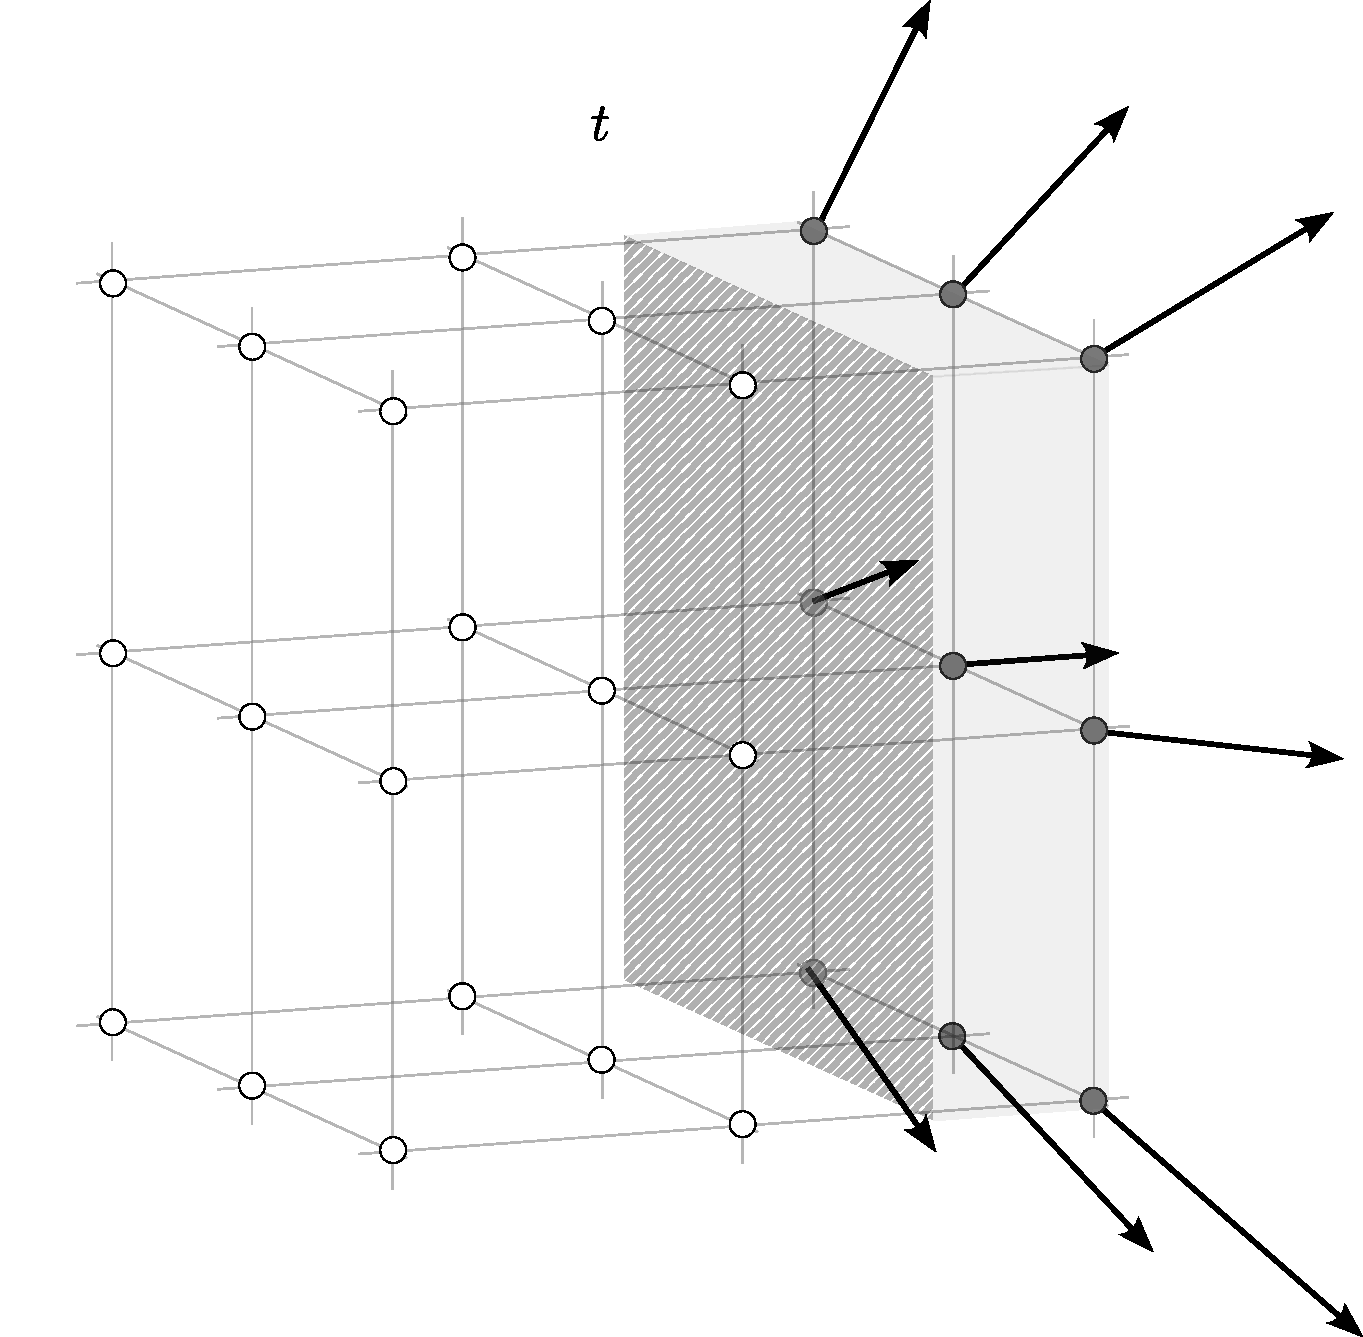
\includegraphics[width=0.9\textwidth, trim={0mm 0mm 0mm 0mm}]{figures/fwbbb.pdf}
		\caption{Step after streaming at time $t$.}
		\label{fig:bbb}
	\end{subfigure}
	\par\bigskip
	\par\bigskip
	\begin{subfigure}{0.48\textwidth}
		\centering
		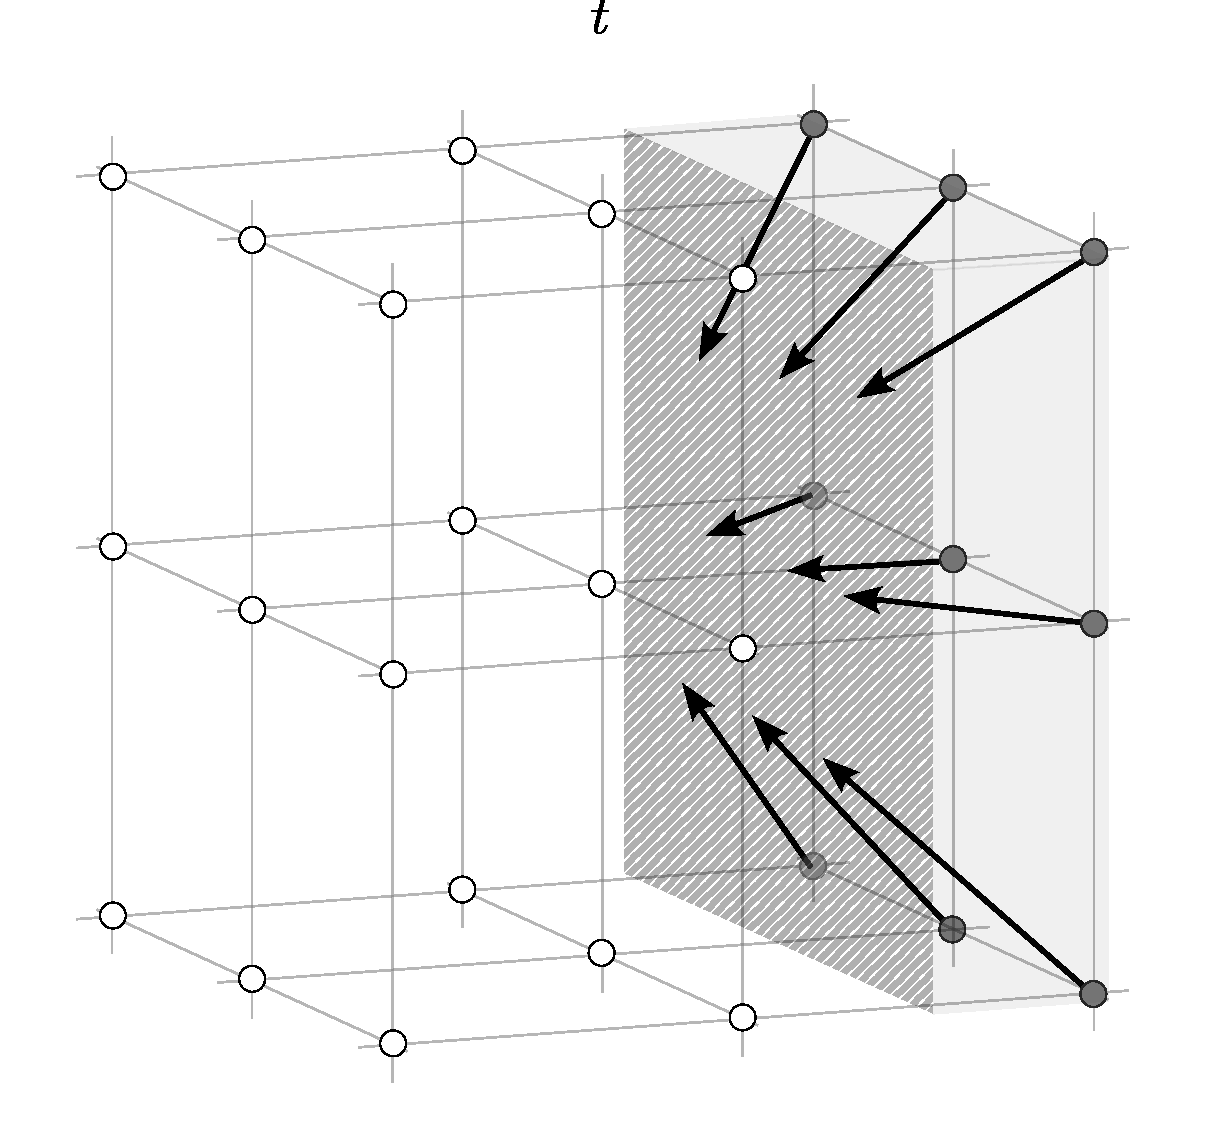
\includegraphics[width=0.9\textwidth, trim={0mm 0mm 0mm 0mm}]{figures/fwbbc.pdf}
		\caption{The distribution functions are reversed.}
		\label{fig:bbc}
	\end{subfigure}
	\begin{subfigure}{0.48\textwidth}
		\centering
		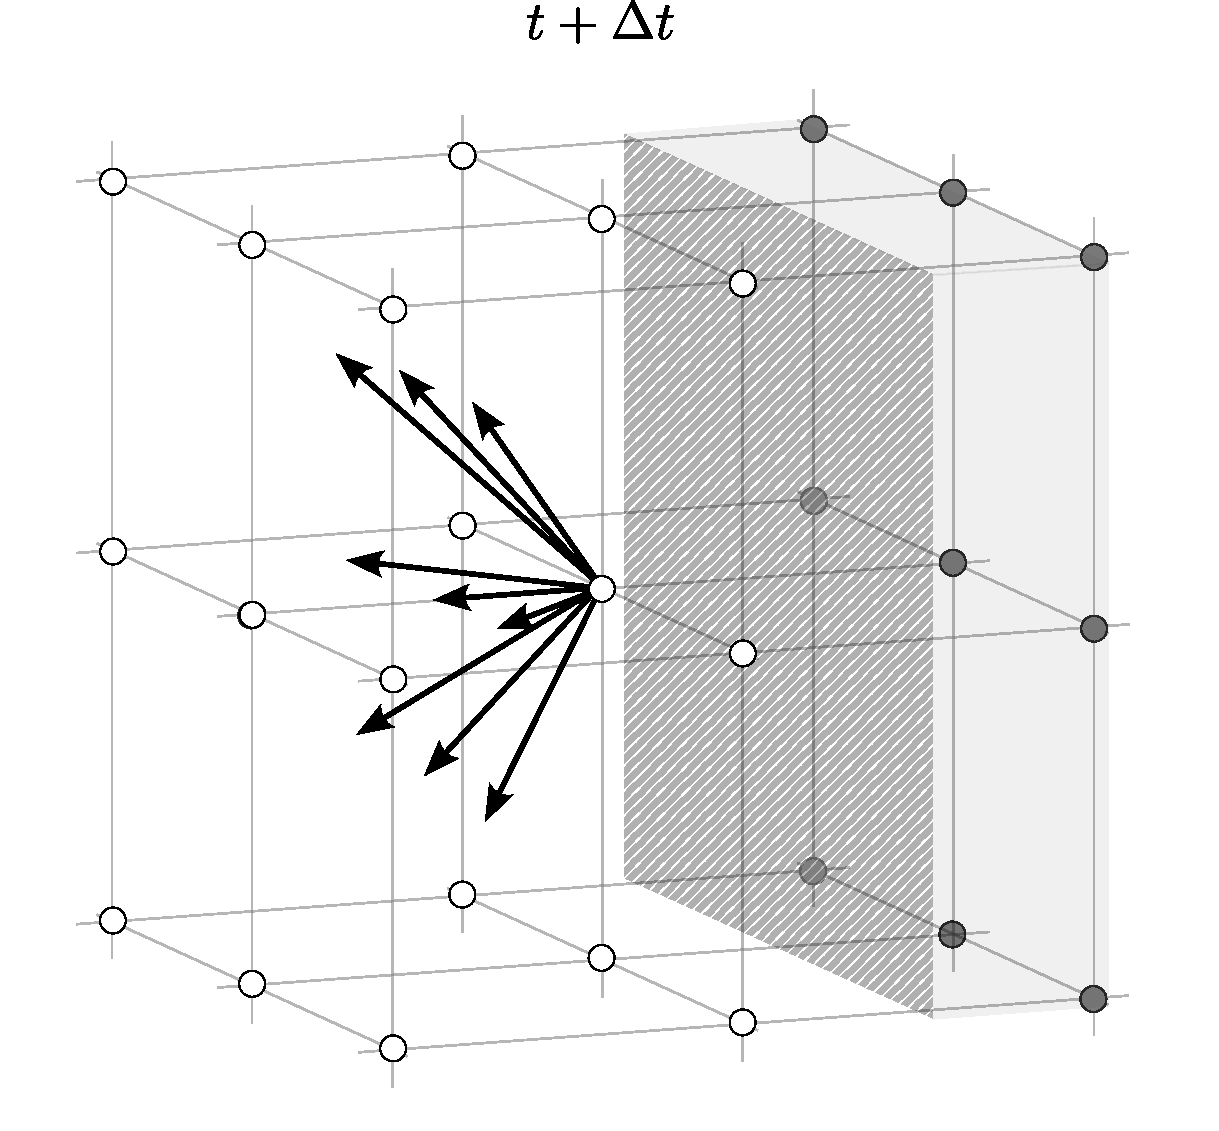
\includegraphics[width=0.9\textwidth, trim={0mm 0mm 0mm 0mm}]{figures/fwbbd.pdf}
		\caption{Step after the streaming at time $t + \Delta t$.}
		\label{fig:bbd}
	\end{subfigure}
	\vspace{5mm}
	\caption{Schematic representation of the fullway bounce-back boundary condition for the D3Q27 velocity model. White points represent fluid nodes, and gray points represent wall nodes. The wall is represented by a gray plane.}
	\label{fig:fbb}
\end{figure}

An alternative to the fullway method is the \textit{halfway} variant of the bounce-back boundary condition, which completes the reflection process within a single time step. Details can be found in \cite{Kruger}. In this work, however, we limit ourselves to the fullway variant.

%\subsubsection{Equilibrium boundary condition}\label{equilibrium bc}
%One option for approximating unknown distribution function values at the boundary nodes is to use the equilibrium distribution function, defined as \cite{PE}
%\begin{equation}
%	f_i(\vec{x}, t)=f_{i}^{\text{(eq)}}(\rho(\vec{x}, t), \vec{u}(\vec{x}, t)), \hspace{2mm}  \forall k \in \{1,\dots,27\}, \forall t \in \hat{\mathcal{I}}.
%\end{equation}
%The advantage of this approximation is its simple implementation, while the disadvantage is the neglect of the non-equilibrium part of the distribution function \cite{PE}.

%\subsubsection{Symmetric boundary condition}\label{symmetric bc}
%The symmetric boundary condition assumes that the domain is symmetric relative to a given mirror plane. This boundary condition can be understood as a bounce-back-like method. The distribution functions leave the boundary node at time $t$, meet the symmetry surface at time $t + \frac{\Delta t}{2}$, where they are mirrored, and return to the fluid nodes at time $t + \Delta t$. The components of the mirrored velocity depend on the normal vector of the symmetry plane, the tangential components of the velocity remain unchanged. The symmetric boundary condition is illustrated in Figure~\ref{fig:symmetric bc}.
%\vspace{2mm}
%\begin{figure}[H]
%	\centering
%	\begin{subfigure}{0.47\textwidth}
%		\centering
%		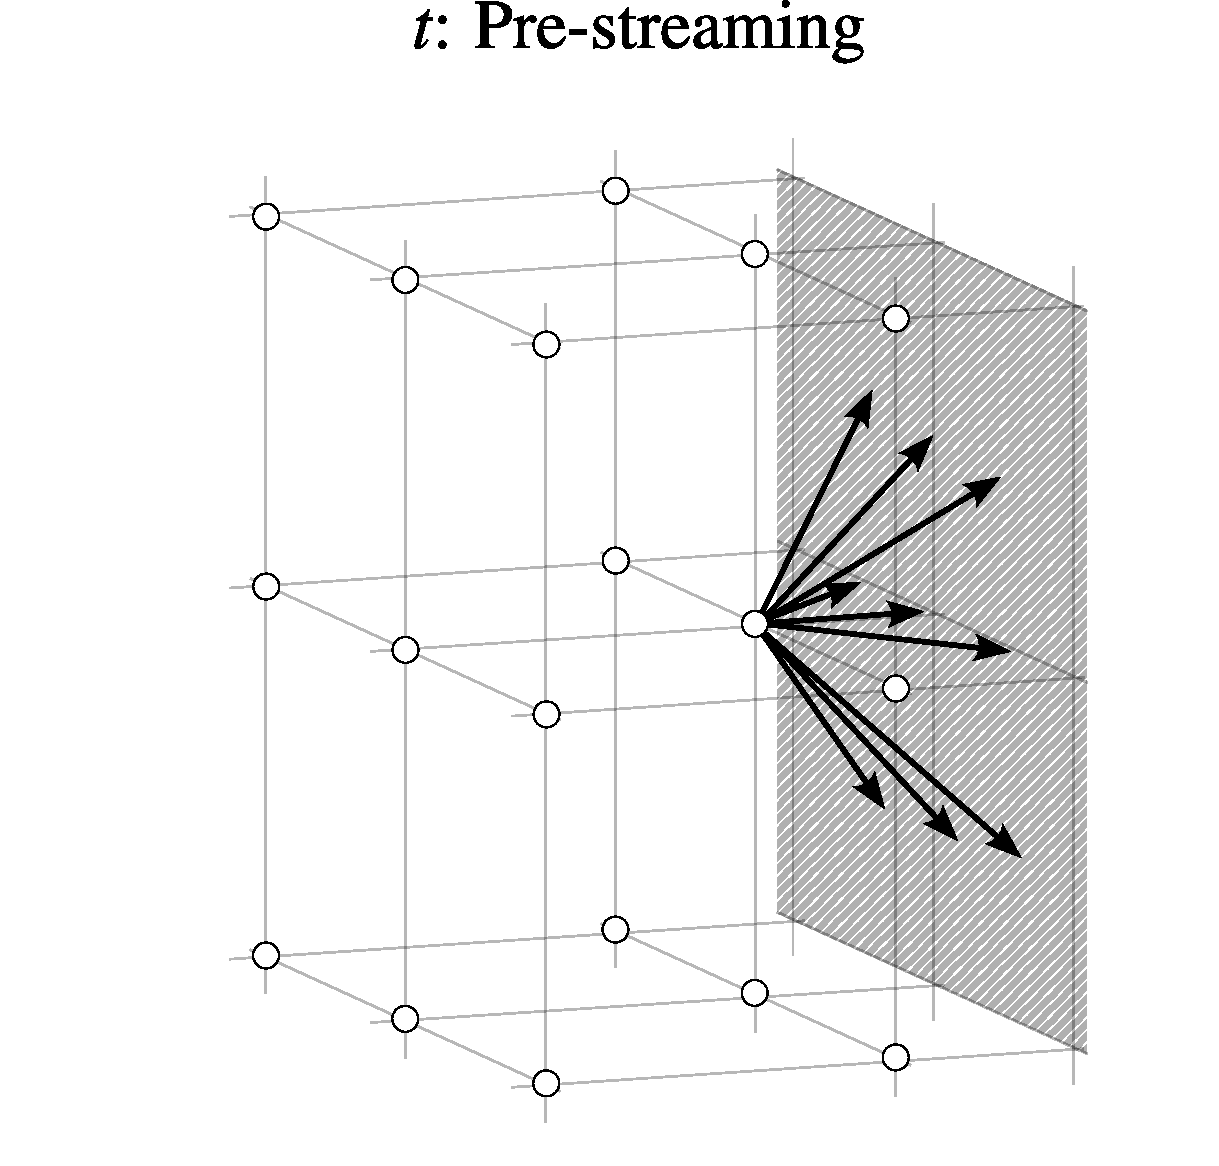
\includegraphics[width=0.99\textwidth, trim={0mm 0mm 0mm 0mm}]{figures/symmetric-a.pdf}
%		\caption{The distribution functions leave the boundary node at time $t$.}
%		\label{fig:sym a}
%	\end{subfigure}\hfill% 
%	\begin{subfigure}{0.47\textwidth}
%			\centering
%			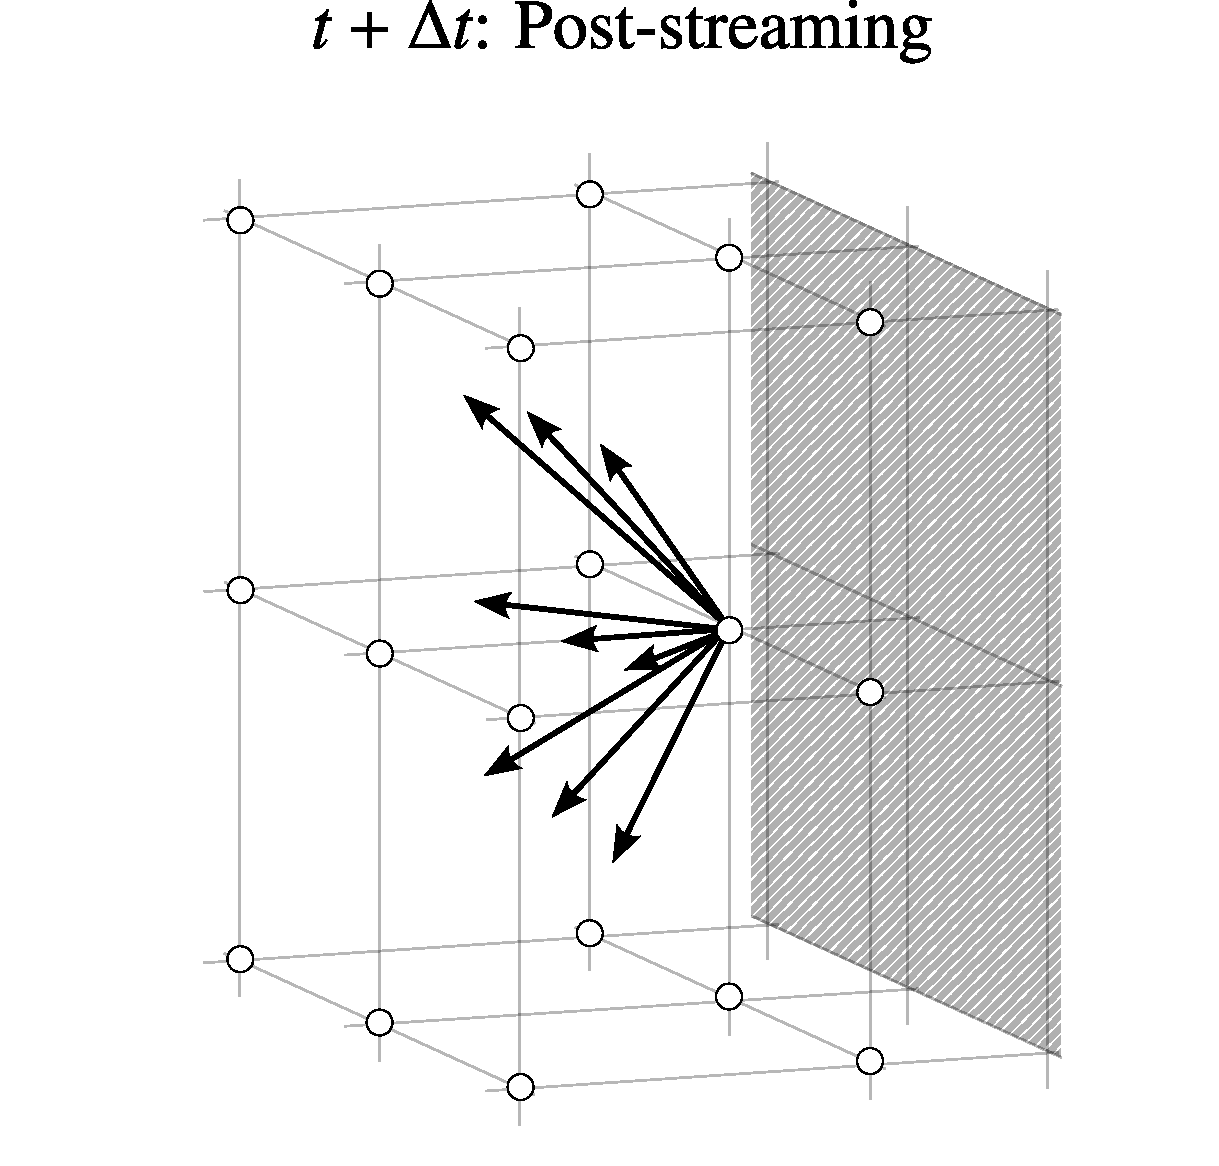
\includegraphics[width=0.99\textwidth, trim={0mm 0mm 0mm 0mm}]{figures/symmetric-b.pdf}
%			\caption{The mirrored distribution functions return to fluid nodes at time $t + \Delta t$.}
%			\label{fig:sym b}
%	\end{subfigure}
%	\vspace{2mm}
%	\caption{Illustration of the symmetric boundary condition for the symmetry plane with the normal vector \( (-1, 0, 0) \) using the D3Q27 velocity model. White points represent fluid nodes, and gray plane resents the symmetry plane.}
%	\label{fig:symmetric bc}
%
%\end{figure}

\subsubsection*{Free outflow boundary condition}\label{symmetric bc}
When using the free outflow boundary condition at the outlets, each distribution function for directions pointing out of the domain is set equal to the value it had at the adjacent node inside the computational domain in the previous timestep. While this boundary condition is numerically stable, its usage can cause unphysical behavior of pressure and velocity field near the outflow boundary. Details on the free outflow boundary condition can be found in \cite{PE}.
\section{Notes on the implementation}\label{poznamky k implementaci LBM}
As mentioned in the introduction, the numerical solution using LBM was based on a code developed at the Department of Mathematics of FNSPE, CTU in Prague, which is used to solve the Navier-Stokes equations for a Newtonian incompressible fluid. The program is implemented in C++ using the TNL library \cite{Oberhuber2021, Klinkovsky2022} and employs parallelization on a GPU using the CUDA platform. The used variant of the lattice Boltzmann method CuLBM is implemented in the code for the D3Q27 model.

For the purposes of this work, the code developed within a previous bachelor's thesis \cite{JB} was extended, in which several modifications were made compared to the code developed at the Department of Mathematics of FNSPE, specifically:
\begin{itemize}
	\item implementation of the stress tensor integration method for force calculation using difference,
	\item implementation of various methods for the local calculation of the stress tensor,
	\item implementation of interpolation boundary conditions,
	\item calculation of monitored quantities and their subsequent output to files.
\end{itemize}

